\label{desenvolvimento_estrutura}
Nesta seção é descrito o detalhamento da solução do módulo de estrutura, resultante das duas primeiras fases,
e o seu projeto e construção, resultante da Fase 03.

\subsection{Detalhamento da Solução}

% O detalhamento da solução para a frente de estrutura pode ser sumarizado nos itens abaixo. A solução completa definida nas
  % Fases 01 e 02 pode ser vista no \href{https://drive.google.com/file/d/0B5InkGKx6O-MR1B3eVYzZFpjQ3c/view?usp=sharing}{Relatório 1}.
% A solução proposta para o módulo mecânico/estrutural está descrita nesta seção.

% \subsubsection*{\textbf{Seleção de materiais e faixas de atuação}}

% \subsubsubsection*{Materiais para a estrutura da bancada}

% A base estrutural da mesa de vibração será composta por cantoneiras de abas iguais. A cantoneira a ser utilizada terá abas iguais e uma bitola de
% 4,76 x 50,8mm, tendo assim um peso de 3,63kg/m. Com esse peso, será atendido o objetivo da base da estrutura de ter um peso elevado a fim de
% que as vibrações do motor não sejam transmitidas para a base da mesa. Tendo em vista que será utilizado 8,89 metros deste material para compor
% a estrutura da base, totalizando assim um peso de 32,27kg atendendo a perspectiva de uma base de peso elevado.

% Além do peso, a cantoneira de tal espessura de aço 1010 atende as especificações do projeto no que tange integridade estrutural, fazendo com que
% a base da mesa não sofra flexão, torção, dentre outros momentos estruturais que levam em conta a integridade da mesa \cite{acos_continente}.

% Fazendo uma comparação com outros materiais verificou-se que a cantoneira é a geometria de material que melhor atende a fabricação da base estrutural
% da mesa. Um perfil retangular vazado fabricado de \textit{metalon} era uma boa opção, porém não atendia os objetivos de obtenção do peso elevado, e da
% boa integridade estrutural. Por se tratar de um aço estrutural de baixas propriedades mecânicas a possibilidade da mesa sofrer flexão ou torção seria
% aumentada. Com base nisso a escolha do material da base da estrutura estará satisfeita com a utilização de cantoneira do tipo abas iguais de aço 1010
% com bitola de 4,76 x 50,8mm.

% A bancada terá 4 molas fixadas nas extremidades da superfície vibratória e na estrutura da base. Essas molas serão usadas com intuito de amortecer
% e absorver a vibração da superfície vibratória para evitar a propagação vibracional e a força compressiva na estrutura, ao mesmo tempo, as molas
% auxiliarão na vibração da superfície superior da mesa \cite{mola_santos}.

% As molas que serão utilizadas terão a composição formada por dois batentes de borracha intermediários. Foram devidamente projetadas para garantir uma
% grande eficácia na eliminação das vibrações para a estrutura, sendo capazes de reduzir em até 95\% a propagação da vibração da superfície vibratória para
% a estrutura \cite{mola_catalogo}.

% A bancada terá 4 pés, de borracha e ferro, para que as vibrações fiquem mais distribuídas e não sobrecarreguem apenas uma aresta.
% Outro fator importante é que os 4 pés juntos suportam ate 100 kg, o que atende as exigências relacionadas a massa estipulada no
% projeto \cite{ferramentas_kennedy}.

% Um desenho técnico do pé da mesa é apresentado na Figura \ref{fig:pe_bancada}.

%     \begin{figure}[!ht]
%       \centering
%       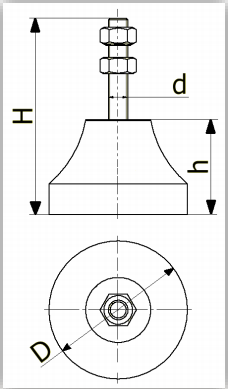
\includegraphics[scale=0.5]{figuras/amortecedor.png}
%       \caption{Desenho técnico do pé da bancada. Fonte: \cite{mola_catalogo}}
%       \label{fig:pe_bancada}
%       \end{figure}

% \subsubsubsection*{Faixas de Atuação}
% A faixa de frequência que a mesa poderá vibrar será de 50 a 100 Hz que equivalem a 3000 a 6000 vibrações por minutos. Essa faixa foi
% escolhida por ser utilizada em mesas vibratórias comerciais \cite{ricardo_jose}.

% \subsubsection*{\textbf{Geometria da mesa}}

%   A mesa de vibração terá uma altura de 900mm e dimensões de 500 x 800mm. Com base nestas características e verificando que se trata de
%   uma mesa com geometria retangular foi elaborado um design estrutural da mesa contendo quatro hastes de cantoneira na vertical com reforços
%   frontais e laterais nas alturas de 350mm e 250mm respectivamente. Tais reforços impedirão com que a estrutura da mesa sofra flexão e torção,
%   além disso, servirá de sustentação para fixação do motor. Uma união das hastes verticais será reforçada através de cantoneiras na parte superior
%   da estrutura, reforçando ainda mais as fixações anti-flambagem da mesa, além de servir de apoio para fixação das molas.

%     Opções de geometria do tipo treliça foram excluídas por não ser de uso convencional para este tipo de aplicação de mesa, além de verificar
%     uma redução do peso da estrutura não haveria apoio para fixação do motor. Considerando que uma base de estrutura pesada é necessária para
%     que não haja transferência de vibração do motor para esta. A Figura \ref{fig:base_bancada} representa um esboço do design estrutural da base
%     projetado no software SOLIDWORKS\footnote{http://www.solidworks.com/}.

% \begin{figure}[!ht]
% \centering
% 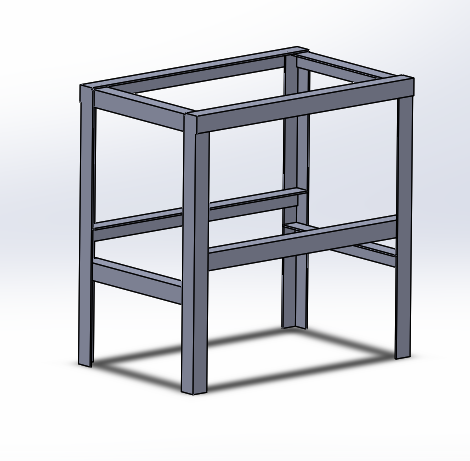
\includegraphics[scale=0.5]{figuras/base_bancada.png}
% \caption{Esboço da base da bancada. Fonte: Autores}
% \label{fig:base_bancada}
% \end{figure}

% \subsubsubsection*{Análise modal}

% Um dos pontos mais importantes da construção de um sistema de vibração mecânica é a região de apoio dos corpos a seres estudados. No caso de uma
% mesa vibratória é o superfície do tampo. Ele deve ser modelado e construído de forma que permita que a frequência de vibração que foi solicitada de
% fato seja a que esteja ocorrendo na base do corpo, ou seja, no tampo da mesa.

%   Uma análise foi feita nesse sentido para gerar um primeiro parâmetro de escolha do material e da geometria do tampo da mesa. Dentre as decisões
%   de projeto que foram feitas estaca a que a geometria da mesa atenderia alguns requisito de mercado. Um deles era que a superfície da mesas possuísse
%   geometria de 800mm de comprimento por 500mm de profundidade gerando uma área útil de 40000 mm$^2$, compatível com concorrentes já existentes.
%   Com isso restou apenas uma última variável a ser decidida, a espessura do tampo.

%   A decisão do tamanho dessa espessura levou em conta duas questões, também decisões de projeto: faixa de vibração entre 50Hz e 100Hz e uso de
%   materiais metálicos para o tampo. Com isso em mente foram feitas análises modais no software de análises Ansys\footnote{www.ansys.com/}, levando
%   em consideração o valor do primeiro modo de vibração. Esse deveria ser, no mínimo, maior que a frequência máxima proposta pela faixa, 100Hz.

%   A análise modal experimental (AME) consiste em extrair os chamados parâmetros modais de um sistema mecânico. Os parâmetros modais são parâmetros
%   característicos do sistema e são compostos por frequências naturais, fatores de amortecimento e modos de vibrar. Se forem corretamente obtidos é
%   possível descrever o comportamento de um sistema vibratório sem necessitar de um modelo matemático \cite{evandro}.

%   Uma análise modal inicial leva em conta somente características físicas do material; rigidez e massa. O que pode ser feito tendo como base a
%   biblioteca de materiais do próprio software.

%   Na simulação a seguir foram feitos dois ensaios com aço estrutural com espessuras diferentes: 5mm e 10mm. E observou-se o valor do primeiro modo
%   de vibração. O aço estrutural conhecido pelo Ansys se compara ao aço comercial SAE 1010 repuxado a frio (CD). Suas características são apresentadas
%   na Tabela \ref{tab:caracteristicas_aco}.

% \begin{table}[!h]
% \centering
% \caption{Características físicas do aço SAE 1010. Fonte: \cite{shigley}}
% \label{tab:caracteristicas_aco}
% \begin{tabular}{|l|l|l|l|}
% \hline
% \multicolumn{1}{|c|}{\textbf{Nº SAE}} & \multicolumn{1}{c|}{\textbf{Processamento}} & \multicolumn{1}{c|}{\textbf{Resistência a tração (Mpa)}} & \multicolumn{1}{c|}{\textbf{Redução de área (\%)}} \\ \hline
% 1010                                  & CD                                          & 320                                                      & 50                                                 \\ \hline
% \end{tabular}
% \end{table}

% As imagens do teste são apresentadas nas Figuras \ref{fig:analise_1} e \ref{fig:analise_2}. A Figura \ref{fig:analise_1} é relativa ao teste
% com espessura de 5mm e a Figura \ref{fig:analise_2} com espessura de 10mm. Foi requerido do programa que revolvesse o seis primeiros modos de vibração.
% Foi somente observado o primeiro. Este deveria ser maior que 100Hz pra evitar ressonância em toda a faixa de uso do equipamento.

% \begin{figure}[!ht]
% \centering
% 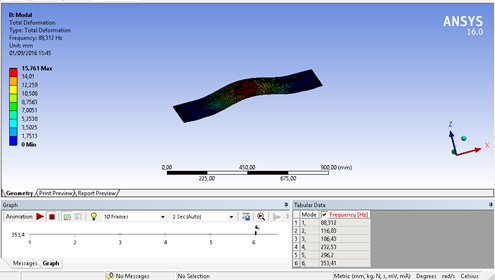
\includegraphics[scale=1]{figuras/analise_1.png}
% \caption{Ensaio com aço estrutural de 5mm de espessura}
% \label{fig:analise_1}
% \end{figure}

% \begin{figure}[!ht]
% \centering
% 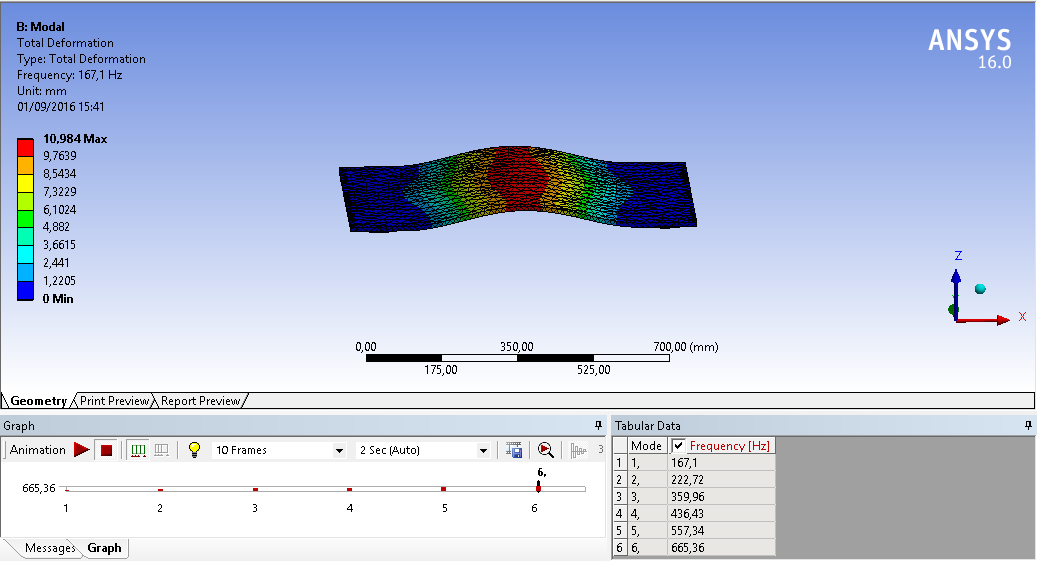
\includegraphics[scale=0.5]{figuras/analise_2.png}
% \caption{Ensaio com aço estrutural de 10mm de espessura}
% \label{fig:analise_2}
% \end{figure}

% Dos testes realizados foi observado que a segunda espessura é a indicada pois oferece segurança em toda a faixa de uso; de 50Hz até 100Hz.
% Pois o primeiro modo de vibração está seguramente acima da frequência máxima. Com um fator de segurança de:

%     \begin{equation}
%             n = 100 Hz/167,1 Hz = 0,6
%     \end{equation}

% Ainda baixo porém já observa-se uma linearidade entre o comprimento da espessura e o valor do primeiro modo de viação.

\subsection{Projeto e Construção}


\subsubsection*{\textbf{Seleção de Materiais e Faixa de Atuação}}

\subsubsubsection*{\textbf{Materiais para a estrutura da bancada}}

A base estrutural da mesa de vibração será composta por cantoneiras de abas iguais. A cantoneira a ser utilizada terá abas iguais e uma bitola de 4,76 x 50,8mm, tendo assim um peso de 3,63kg/m. Com esse peso, será atendido o objetivo da base da estrutura de ter um peso elevado afim de que as vibrações do motor não sejam transmitidas para a base da mesa. Tendo em vista que será utilizado 8,89 metros deste material para compor a estrutura da base, totalizando assim um peso de 32,27kg atendendo a perspectiva de uma base de peso elevado.

Além do peso, a cantoneira de tal espessura de aço 1010 atende as especificações do projeto no que tange integridade estrutural, fazendo com que a base da mesa não sofra flexão, torção, dentre outros momentos estruturais que levam em conta a integridade da mesa \cite{acos_continente}.

Fazendo uma comparação com outros materiais verificou-se que a cantoneira é a geometria de material que melhor atende a fabricação da base estrutural da mesa. Um perfil retangular vazado fabricado de \textit{metalon} era uma boa opção, porém não atendia os objetivos de obtenção do peso elevado, e da boa integridade estrutural. Por se tratar de um aço estrutural de baixas propriedades mecânicas a possibilidade da mesa sofrer flexão ou torção seria aumentada. Com base nisso a escolha do material da base da estrutura estará satisfeita com a utilização de cantoneira do tipo abas iguais de aço 1010 com bitola de 4,76 x 50,8mm.

    A bancada terá 4 molas fixadas nas extremidades da superfície vibratória e na estrutura da base. Essas molas serão usadas com intuito de amortecer e absorver a vibração da superfície vibratória para evitar a propagação vibracional e a força compressiva na estrutura, ao mesmo tempo, as molas auxiliarão na vibração da superfície superior da mesa \cite{mola_santos}.

    A bancada terá 4 pés, de borracha e ferro, para que as vibrações fiquem mais distribuídas e não sobrecarreguem apenas uma aresta. Outro fator importante é que cada pé é capaz de suportar até 70Kg.A estrutura da bancada sustentada pelos quatro pés citados anteriormente podem suportar uma carga máxima de 280kg, o que atende as exigências relacionadas a massa estipulada no projeto, tendo em vista que o peso total do projeto consistem em valores menores aos a carga máxima suportada pelos pés estruturais \cite{ferramentas_kennedy}.

    Um desenho técnico do pé da mesa é apresentado na Figura \ref{fig:pe_bancada}.

    \begin{figure}[H]
      \centering
      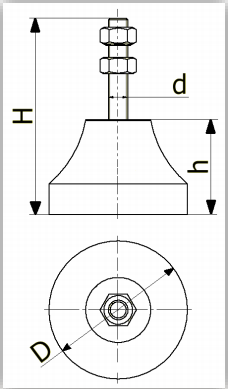
\includegraphics[scale=0.5]{figuras/amortecedor.png}
      \caption{Desenho técnico do pé da bancada. Fonte: \cite{mola_catalogo}}
      \label{fig:pe_bancada}
      \end{figure}


\subsubsubsection*{\textbf{Faixas de Atuação}}
A faixa de frequência que a mesa poderá vibrar será de 50 a 100 Hz que equivalem a 3000 a 6000 vibrações por minutos. Essa faixa foi escolhida por ser utilizada em mesas vibratórias comerciais \cite{ricardo_jose}.

\subsubsection*{\textbf{Geometria da Bancada}}

\subsubsubsection*{\textbf{Design}}

    A mesa de vibração terá uma altura de 900mm e dimensões de 500 x 800mm. Com base nestas características e verificando que se trata de uma mesa com geometria retangular foi elaborado um design estrutural da mesa contendo quatro hastes de cantoneira na vertical com reforços frontais e laterais nas alturas de 350mm e 250mm respectivamente. Tais reforços impedirão com que a estrutura da mesa sofra flexão e torção, além disso, servirá de sustentação para fixação do motor. Uma união das hastes verticais será reforçada através de cantoneiras na parte superior da estrutura, reforçando ainda mais as fixações anti-flambagem da mesa, além de servir de apoio para fixação das molas.

    Opções de geometria do tipo treliça foram excluídas por não ser de uso convencional para este tipo de aplicação de mesa, além de verificar uma redução do peso da estrutura não haveria apoio para fixação do motor. Considerando que uma base de estrutura pesada é necessária para que não haja transferência de vibração do motor para esta. A Figura \ref{fig:base_bancada} representa um esboço do design estrutural da base projetado no software SOLIDWORKS\footnote{http://www.solidworks.com/}.

\begin{figure}[H]
\centering
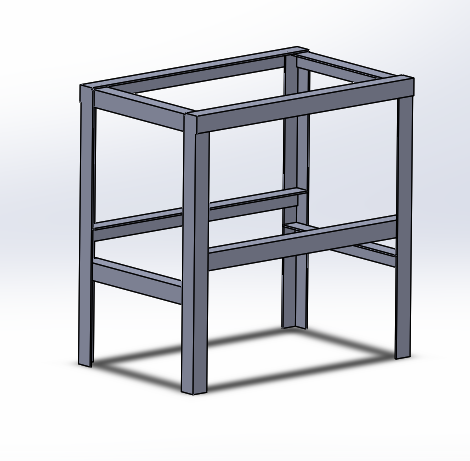
\includegraphics[scale=0.5]{figuras/base_bancada.png}
\caption{Esboço da base da bancada. Fonte: Autores}
\label{fig:base_bancada}
\end{figure}

\subsubsection*{\textbf{Análises}}

    Um dos pontos mais importantes da construção de um sistema de vibração mecânica é a região de apoio dos corpos a seres estudados. No caso de uma mesa vibratória é o superfície do tampo. Ele deve ser modelado e construído de forma que permita que a frequência de vibração que foi solicitada de fato seja a que esteja ocorrendo na base do corpo, ou seja, no tampo da mesa.

    Uma análise foi feita nesse sentido para gerar um primeiro parâmetro de escolha do material e da geometria do tampo da mesa. Dentre as decisões de projeto que foram feitas estaca a que a geometria da mesa atenderia alguns requisito de mercado. Um deles era que a superfície da mesas possuísse geometria de 800mm de comprimento por 500mm de profundidade gerando uma área útil de 40000 mm$^2$, compatível com concorrentes já existentes. Com isso restou apenas uma última variável a ser decidida, a espessura do tampo.

    A decisão do tamanho dessa espessura levou em conta duas questões, também decisões de projeto: faixa de vibração entre 50Hz e 100Hz e uso de materiais metálicos para o tampo. Com isso em mente foram feitas análises modais no software de análises Ansys\footnote{www.ansys.com/}, levando em consideração o valor do primeiro modo de vibração. Esse deveria ser, no mínimo, maior que a frequência máxima proposta pela faixa, 100Hz.

    A análise modal experimental (AME) consiste em extrair os chamados parâmetros modais de um sistema mecânico. Os parâmetros modais são parâmetros característicos do sistema e são compostos por frequências naturais, fatores de amortecimento e modos de vibrar. Se forem corretamente obtidos é possível descrever o comportamento de um sistema vibratório sem necessitar de um modelo matemático \cite{evandro}.

    Uma análise modal inicial leva em conta somente características físicas do material; rigidez e massa. O que pode ser feito tendo como base a biblioteca de materiais do próprio software.

    Na simulação a seguir foram feitos dois ensaios com aço estrutural com espessura de 4,7625mm. O aço estrutural conhecido pelo Ansys se compara ao aço comercial SAE 1010 repuxado a frio (CD). Suas características são apresentadas na Tabela \ref{tab:caracteristicas_aco}.

\begin{table}[H]
\centering
\caption{Características físicas do aço SAE 1010. Fonte: \cite{shigley}}
\label{tab:caracteristicas_aco}
\begin{tabular}{|l|l|l|l|}
\hline
\multicolumn{1}{|c|}{\textbf{Nº SAE}} & \multicolumn{1}{c|}{\textbf{Processamento}} & \multicolumn{1}{c|}{\textbf{Resistência a tração (Mpa)}} & \multicolumn{1}{c|}{\textbf{Redução de área (\%)}} \\ \hline
1010                                  & CD                                          & 320                                                      & 50                                                 \\ \hline
\end{tabular}
\end{table}

\subsubsubsection*{\textbf{Análise estrutural}}

    A análise da estrutura da bancada tem como intuito determinar os efeitos das cargas aplicadas sobre a mesma e, assim, os resultados serão usados para examinar se a estrutura está apta para o uso.

    Essa análise foi feita no software Ansys a partir do design da estrutura projetada no software SOLIDWORKS\footnote{http://www.solidworks.com/}. Os esforços de maiores relevâncias para a estrutura são os pesos da chapa superior e do motor. A partir disso, realizou-se a simulação estrutural colocando como esforços as forças peso da chapa e do motor, conforme indicado na Fig. \ref{fig:an_estrutural}.

  \begin{figure}[H]
      \centering
      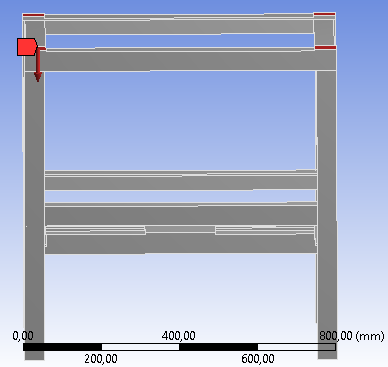
\includegraphics[scale=0.7]{figuras/an_estrutural.png}
      \caption{Peso da chapa superior aplicada na estrutura. Fonte: Autores}
      \label{fig:an_estrutural}
      \end{figure}

    A carga relacionada ao peso do motor foi aplicada na estrutura afim de verificar a deformação máxima que este carregamento pode causar na estrutura. A  Figura\ref{fig:carga_motor} ilustra a carga aplicada atraves da ferramenta computacional ANSYS\footnote{www.ansys.com/}.

  \begin{figure}[H]
      \centering
      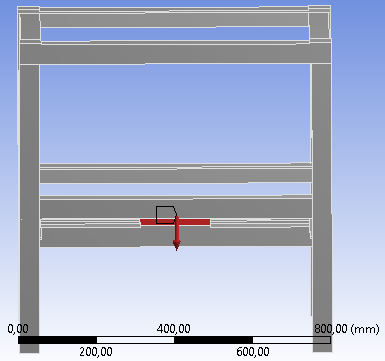
\includegraphics[scale=0.7]{figuras/carga_motor.png}
      \caption{Peso do motor aplicado na estrutura. Fonte: Autores}
      \label{fig:carga_motor}
      \end{figure}

      Com os esforços definidos, o programa computa automaticamente todos os cálculos estruturais necessários a partir das cargas aplicadas. Os resultados estão mostrados na fig. \ref{fig:def_motor}.

  \begin{figure}[H]
      \centering
      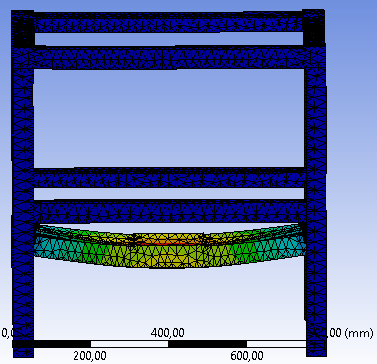
\includegraphics[scale=0.7]{figuras/def_motor.png}
      \caption{Deformação total devido aos esforços aplicados. Fonte: Autores}
      \label{fig:def_motor}
      \end{figure}

      Os resultados da simulação para deformação máxima da estrutura sob o carregamento do peso do motor  são ilustrados pela Fig.\ref{fig:result}.

  \begin{figure}[H]
      \centering
      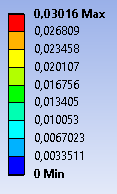
\includegraphics[scale=0.7]{figuras/result.png}
      \caption{Resultado da deformação - Escala em mm. Fonte: Autores}
      \label{fig:result}
      \end{figure}

      Pelas Figuras \ref{fig:def_motor} e \ref{fig:result}, percebe-se que o peso do motor é o responsável pela maior deformação da estrutura, mas essa deformação é praticamente desprezível por ser extremamente pequena, 0,03 mm. Então a estrutura mostrou-se apta e segura para a utilização.
    Com o intuito de ter um maior grau de segurança para validar a estrutura, diversas simulações foram feitas aumentando os valores das cargas aplicadas e as deformações continuaram desprezíveis comprovando que a estrutura é válida para o projeto.

\subsubsubsection*{\textbf{Análise modal da estrutura}}

    Uma vez que o projeto se trata de uma bancada vibratória, é de suma importância analisar o comportamento da estrutura submetido a vibração. A análise modal da estrutura foi feita no software Ansys e observou-se o primeiro modo de vibração para validar a utilização da mesma.
    A maior influência vibracional na estrutura é do motor, pelo fato do mesmo estar fixado diretamente na estrutura da mesa. A tampa superior não terá tanta relevância quanto o motor por causa das molas que amorteceram grande parte da propagação da vibração.
    O primeiro modo de vibração da estrutura está representado na figura abaixo e corresponde a um valor de 65,83 Hz.
    Analisando a Fig.\ref{fig:vib_estrutura}, percebe-se a importância dos reforços horizontais no eixo x, pois a tendência de movimento desse modo de vibração é ao longo do mesmo eixo e os reforços proporcionam uma maior rigidez para esse movimento.

  \begin{figure}[H]
      \centering
      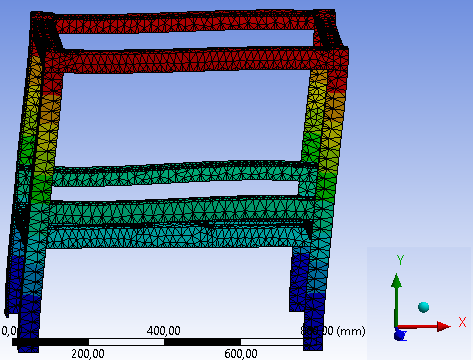
\includegraphics[scale=0.6]{figuras/vib_estrutura.png}
      \caption{Primeiro modo de vibração da estrutura. Fonte: Autores}
      \label{fig:vib_estrutura}
      \end{figure}

      Dado que o motor tem maior influência na estrutura e mesmo possui uma vibração máxima de 60 Hz e o primeiro modo de vibração foi superior a esse valor, então a estrutura está validada. Para aumentar ainda mais o valor do primeiro modo de vibração, instalou-se pés vibra-stop na estrutura e, assim, o grau de segurança da mesma submetida a vibração foi ampliado.

\subsubsubsection*{\textbf{Análise modal do tampo}}

    Tendo em vista que a rotação máxima do eixo para atender as especificações do projeto seja de 6000 rotações por minuto ou 100Hz a plataforma superior da bancada não poderá ter frequência de ressonância menor que 100Hz. Para validação do mesmo foram elaborados ensaios na plataforma ANSYS\footnote{www.ansys.com/} afim de verificar a frequência de ressonância do tampo.

    A Figura\ref{fig:tampo} mostra que a frequência de ressonância do tampo é superior ao esperado(100Hz) podendo chegar até 106Hz e com isso a validação da escolha deste material. A deformação máxima do tampo corresponde a 13mm.

  \begin{figure}[H]
      \centering
      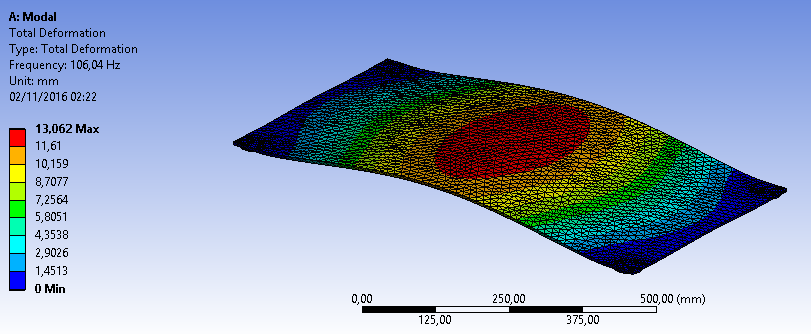
\includegraphics[scale=0.6]{figuras/tampo.png}
      \caption{Análise modal do tampo. Fonte: Autores}
      \label{fig:tampo}
      \end{figure}

\subsubsection*{\textbf{Dimensionamento das Molas}}

Para o presente projeto foram utilizadas quatro molas de comando de válvulas de cabeçote de motor de combustão interna. A escolha desse tipo de mola se deve ao fato de possuír vida infinita em uso sendo, por isso, usada nessas função pela indústria automotiva. Geralmente feitas de liga de Cromo e Vanádio, comandos de válvulas giram em torno de 2000 rotações por segundo por longos períodos de tempo, qualquer falha durante o uso terá consequências catastróficas para funcionamento do motor. A  Figura\ref{fig:mola} ilustra uma mola de comando de válvula utilizada em motor de automóveis.

\begin{figure}[H]
\centering
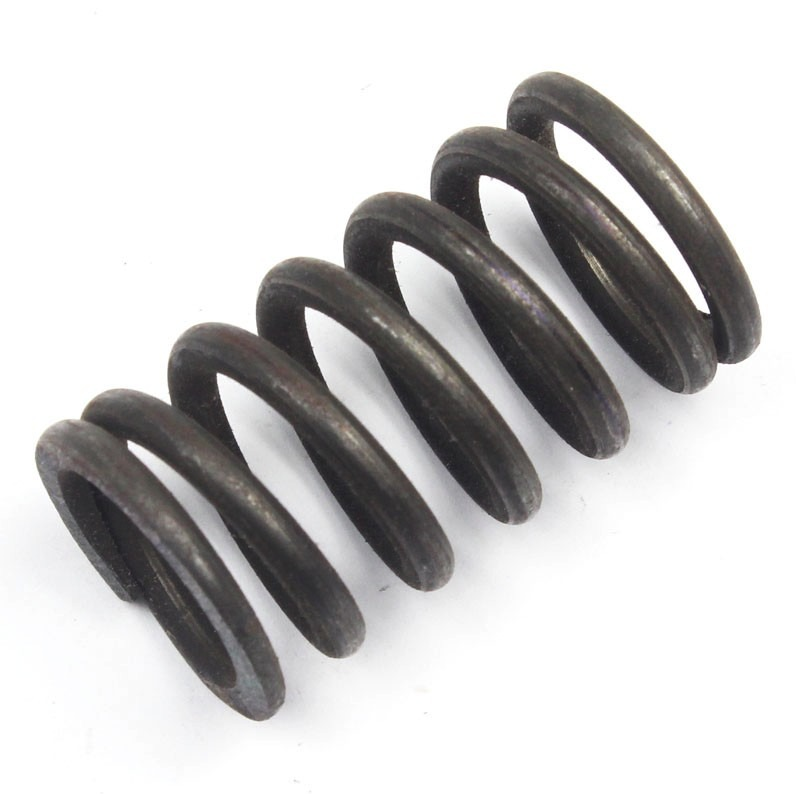
\includegraphics[scale=0.3]{figuras/mola.png}
\caption{Mola de comando de válvula. Fonte: Mercedes Rio Diesel}
\label{fig:mola}
\end{figure}

No projeto da mesa vibratória foram usadas 4 molas de comando de cabeçote uma em cada extremidade do tampo. Suas dimensões são:
\begin{itemize}
\item Comprimento: 45mm
\item Diâmetro do fio da mola: 3mm
\item Diâmetro da mola (diâmtro externo): 23,5mm
\item Número de espiras ativas 5.
\end{itemize}

O uso de molas de comando de válvula, seja em um motor, seja na mesa vibratória do projeto do grupo é sempre em compressão. Molas de compressão possuem suas extremidades usinadas reduzindo o número de espiras ativas e contribuindo para armazenar mais energia na mola.
Um dos principais requisitos do projeto foi a operação da mesa em uma faixa de frequência que se estende entre 70 Hz e 100Hz. Sabendo que um Hertz é um ciclo por segundo a máquina opera entre 70 ciclos por segundo e 100 ciclos por segundo daí constata-se que a cada ciclo dura entre:

$$t_{min} (segundos)=\frac{1segundo}{70 ciclos/segundo}=0.0143$$
$$t_{max} (segundos)=\frac{1segundo}{100 ciclos/segundo}=0.0100$$

Para movimento rotativo usa-se, para cálculo de deslocamento da extremidade da mola, a expressão:

$$deslocamento=amplitude \cos(wt)$$

Onde t é o tempo e ômega é a velocidade angular da superfície superior da mola por tempo (todos em segundos).

$$\omega=\frac{2\pi}{t_{ciclo}}$$

Será usado o tempo para 100 Hz por ser o menor, mais exigente. Logo:

$$\omega=\frac{2\pi}{t_{max}}=\frac{2\pi}{0,001s}=628,3rad/s$$

Para encontrarmos a aceleração diferenciamos duas vezes a formula do deslocamento:

$$deslocamento=amplitude * \cos(\omega t)$$
$$aceleração=-\omega^2 * amplitude * \cos(\omega t)$$

A aceleração máxima ocorre quando o termo $\cos(\omega t)$ equivale a 1, a situação mais extrema de operação. O deslocamento máximo, amplitude do movimento, foi decidido que será de 10 mm (0,01 metro). Com essa informação em mãos pode-se calcular a aceleração máxima:


$$aceleração =628,3^2 * 0,01 *1 =3948m/s^2 $$

Tendo em mãos o valor da aceleração é possível calcular a força que cada mola recebe. O tampo pesa exatamente 15.31 kg. Como as molas estão a mesma distância do centro de massa do tampo, pode-se afirmar que cada mola apoia um quarto desse valor, 3,83 kg. O peso máximo dos elementos que serão estudados sob a mesma são passa de 10kg e devem ser sempre apoiado no centro geométrico da mesma. Dessa forma cada mola suporta, devido ao corpo, no máximo, 3.33kg.

$$ F=m*a=(3,83+3,33)kg*3948m/s^2$$
$$ F=7,157kg*3948m/s^2$$
$$F=28257,81kg m/s^2$$
$$F\approx 28kN$$

O diâmetro médio (D) de molas é dado pela equação:

$$D=d_{ext}-d_{fio}$$
$$D=23,5mm-3mm=20,5mm$$

Com os valores dos dois diâmetros também é calculado o índice de mola, uma medida adimencional de curvatura da espiral da mola.

$$C=\frac{D}{d_{fio}}$$
$$C=\frac{20,5mm}{3mm}=6,834$$

Econtrando o valor de \textit{Bergsträsser}

$$K_B=\frac{4C+2}{4C-3}=\frac{4*6,834+2}{4*6,834-3}$$
$$K_B=1,2054,$$

Pode-se agora calcular a força limite, por segurança, para a mola atingir seu comprimento sólido. Ou seja, a força que, se exercida sob a mola, ocasionará contato entre suas espiras.

$$F_s=\frac{\pi d^3 \alpha}{8 K_B D}$$ onde $$\alpha=\frac{S_{sy}}{n_s}$$

Fs depende do material que é utilizado para confeccionar a mola, no caso de molas de comando de válvula, como informado, são feitas de Ligas de Cromo e Vanádio.

Em teoria de projeto de molas a tensão última de um material pode ser encontrada por uma relação entre o seu diâmetro, um expoente tabelado e uma característica físicas, pela fórmula:

$$S_{ut}=\frac{A}{d^m}$$

Para o Cromo Vanádio tem-se, de acordo com Shigley (Projeto de Engenharia Mecânica 7ª Edição, pg 496 e 497 as características apresentadas na Tabela \ref{tab:caracteristicas_cromovanadio}.

\begin{table}[H]
    \begin{tabular}{|p{2cm}|p{2cm}|p{2cm}|p{2cm}|p{2cm}|p{2cm}|}
        \hline
        \textbf{Material} & \textbf{Número ASTM} & \textbf{Expoente} & \textbf{Diâmetro do fio (mm)} & \textbf{A (MPa $mm^{mm}$)} & \textbf{G(GPa)} \\ \hline
        Fio de cromo-vanádio& A232& 0,168& 3&2005 &77,2                                                 \\ \hline
    \end{tabular}
    \caption{Características físicas do aço Cromo-Vanádio. Fonte: \cite{shigley}}
    \label{tab:caracteristicas_cromovanadio}
\end{table}


Contendo assim:

$$S_{ut}=\frac{2005}{3^{0,168}}=1667,1MPa$$

\textit{Shigley} também afirma que, para molas de cromo-vanádio:

$$S_{sy}=S_{ut}*0,5$$
$$S_{sy}=1667,1*0,5=S_{sy}=833,5MPa$$

Utilizando fator de segurança de 1,2:

$$\alpha=\frac{833,5MPa}{1,2}=694,6MPa$$

Retomando a fórumula:

$$F_s=\frac{\pi d^3 \alpha}{8 K_B D} = \frac{\pi * 3mm^3 * 694,6MPa}{8*1,2054 * 20,5mm}=298,01kN$$

Esse valor define a dimensão máxima da força que cada mola pode receber para que suas expiras se toquem. Sabendo que cada mola na mesa recebe 28kN de força, conclui-se:
\begin{itemize}
\item As molas suportam o limite máximo de carga sub a mesa: 10kg
\item Sob frequencia máxima definida de 100Hz.
\item Com fator de segurança muito alto: $n=\frac{F_S}{28kN}$
\end{itemize}

A rigidez (k) ou razão de mola é um parâmetro muito importante no projeto de uma mola mecânica. A teria informa que:

$$k \frac{d^4G}{8 D^3N_a}$$

A constante Na refere-se ao número de espiras ativas na mola, 5 e G é um valor tabelado conhecido do material da mola. No caso de fio de cromo-vanádio, G=77,2GPa

$$k=\frac{3mm^4 77,2GPa}{8*20,5mm^3*5}=18145N/m^2$$

Essa informação é importante para as simulações dinâmicas da mesa e tampo em softwares computacionais.  Mas é principalmente usada em considerações sobre frequência de ressonância dentro das situações de uso. Para o projeto da mesa, frequências de uso entre 70Hz e 100Hz. A fórmula a seguir apresenta, em função da razão de mola, as frequências que uma mola entra em ressonância se excitada entre placas paralelas.

$$\omega=m\pi \sqrt{\frac{k*g}{W}}$$

g é a aceleração da gravidade, W o peso da mola e m é o número do harmônico calculado, sendo m=1 o a frequência fundamental.

$$W=\frac{\pi^2 d^2 D N_a \gamma}{4}$$
$$\gamma=7,86*10^{-3}kg/mm^3$$
$$W=17,8897N$$
$$\omega=1\pi \sqrt{\frac{0,018145N/mm 9180mm/s^2}{17,8897}}$$

A mola empregada na construção da mesa passa bem pelas exigências do projeto, respeitando a os requisitos de carga e frequência de utilização, já que o seu primeiro harmônico é superior ao 109 va lor máximo de 100Hz requerido pelo projeto.

\subsubsection*{\textbf{Fixações}}

    Tendo em vista que a problemática do projeto consiste em produzir vibrações, é de suma importância uma boa projeção das fixações que envolvem o projeto como um todo. Tais fixações devem ser atentadas para que não haja falhas ou até mesmo perda de funcionalidade de componentes. Nos tópicos seguintes são discutidas como serão as fixações bem como suas respectivas justificativas.

\subsubsubsection*{\textbf{Fixação dos pés}}

    Os pés de borracha que sustentam a estrutura do projeto consistem em fixação por parafuso e porca. Para que esta fixação não comprometa a integridade da estrutura, foram elaborados apoios com furação iguais aos das roscas dos pés, as quais são de meia polegada. Além disso, como o projeto consiste em constantes vibrações sobre a estrutura, foram realizados travamento para que as porcas não venham folgar ou até mesmo soltar ao longo do tempo. Tendo em vista este problema a fixação é feita por duas porcas na parte superior da estrutura, como podemos ver na Fig.\ref{fig:config_pes} A fim de ajustar erros de construção obtidos pela solda da estrutura a qual provocou desnível na mesma foram colocadas arruelas na medida certa até que houvesse o nivelamento da estrutura.

    \begin{figure}[H]
      \centering
      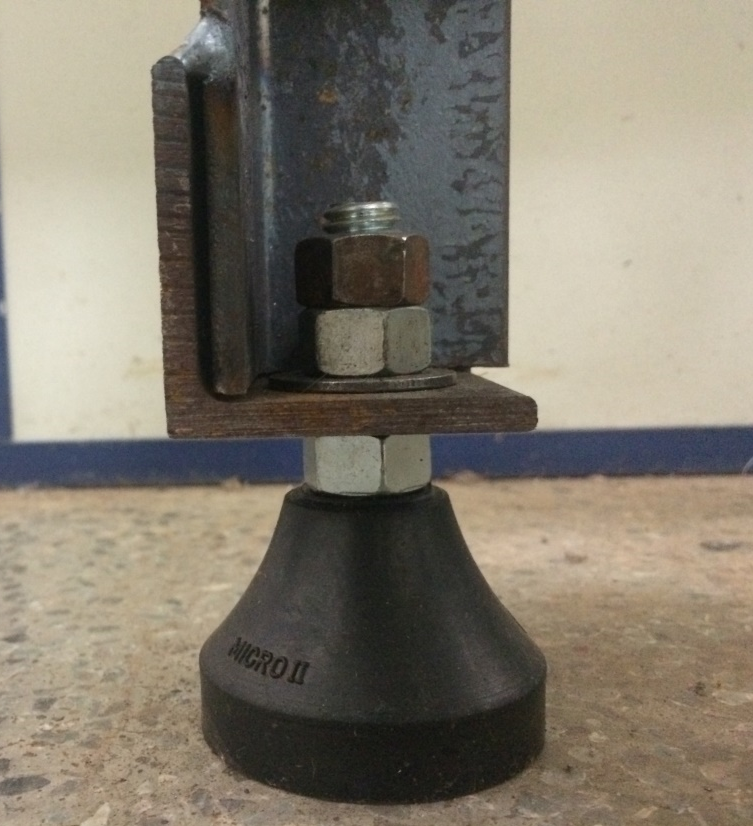
\includegraphics[scale=0.4]{figuras/config_pes_jpg.png}
      \caption{Configuração da fixação dos pés. Fonte: Autores}
      \label{fig:config_pes}
      \end{figure}

\subsubsubsection*{\textbf{Fixação do motor}}

    O motor de indução trifásico do tipo gaiola o qual poderá exercer frequências de até 60Hz sobre a estrutura é fixado a partir de parafusos, arruelas de pressão e porcas. Como a constância de vibração do motor exercido sobre a estrutura é alta a necessidade de colocar coxins entre a carcaça do motor e a estrutura foi um ponto crucial para o projeto, absorvendo assim as vibrações do motor para com a estrutura. Para que as porcas não venham a folgar ou até mesmo soltar durante o funcionamento do motor foram colocadas arruelas de pressão, garantindo assim com que o conjunto parafuso e porca fique fixo e não se soltem a longo prazo.

\subsubsubsection*{\textbf{Fixação das molas}}

    As molas são os componentes mais delicados do projeto, tendo em vista que será o componente que mais sofrerá esforço. Com base nisto é de suma importância estar atento a todos os detalhes deste item do projeto. Para que não haja falha das molas, é de entendimento que tais componentes não podem ser soldados na estrutura, para que o projeto atenda tais requisitos as molas são fixadas na estrutura através de interferência do diâmetro interno da mola para com copinhos de fixação que foram projetados pelos próprios autores. Para que não houvesse solda entre os copinhos com a estrutura foram elaboradas chapas de sustentação dos copinhos, nos quais tem furação para que a solda fosse elaborada por baixo dos copinhos. Para melhor entendimento a Fig.\ref{fig:config_copinhos} ilustra a configuração dos copinhos.

\begin{figure}[H]
\centering
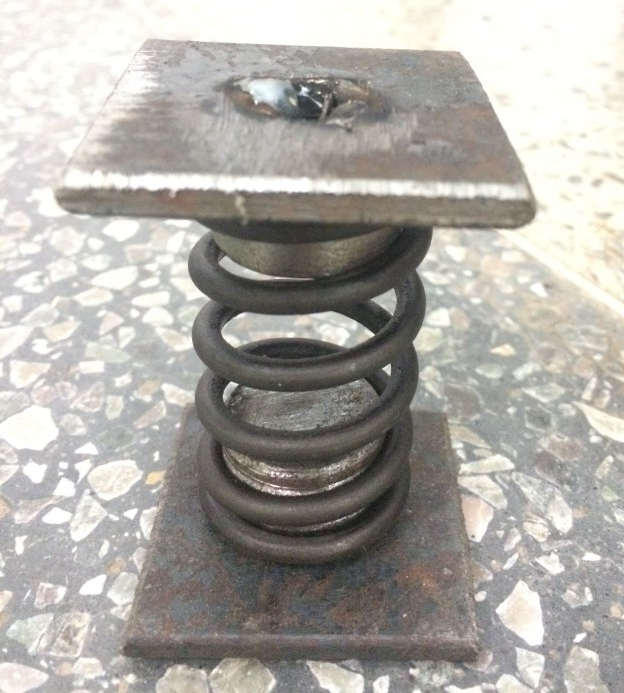
\includegraphics[scale=0.5]{figuras/config_copinhos.png}
\caption{Configuração das molas. Fonte: Autores}
\label{fig:config_copinhos}
\end{figure}

\subsubsection*{\textbf{Sistema de Transmissão}}

\subsubsubsection*{\textbf{Polias e correias}}

    As polias são peças cilíndricas, movimentadas pela rotação do eixo do motor e pelas correias. Os tipos de polia são determinados pela forma da superfície na qual a correia se assenta. Correias são elementos de máquinas que transmitem movimento de rotação entre dois eixos (motor e movido) por intermédio de polias. Elas são empregadas quando se pretende transmitir potência de um veio para o outro a uma distância em que o uso de engrenagens é inviável. Para o sistema em questão será usada as polias do tipo Trapezoidal ou V múltipla.

    A correia em V ou trapezoidal é inteiriça, fabricada com seção transversal em forma de trapézio. É feita de borracha revestida de lona e é formada no seu interior por cordonéis vulcanizados para suportar as forças de tração. O emprego da correia trapezoidal ou em V é preferível ao da correia plana pelos seguintes motivos: Praticamente não apresenta deslizamento; Permite o uso de polias bem próximas; Elimina os ruídos e os choques, típicos das correias emendadas (planas).

    Como as correias têm características diferentes de fabricante para fabricante, é aconselhável seguir as instruções que eles forneçam. A partir destes elementos pretende-se selecionar a polia do tipo guia com correia do tipo trapezoidal a ser usada observando o tipo, a secção e o comprimento primitivo, potência a ser transmitida, tipos de máquina motoras e movidas, velocidade angular da polia motora e da polia movida, distância entre os eixos da polia motora e da polia movida, distância entre os eixos das polias, na qual o comprimento máximo admitido deve ser igual a três o produto da soma dos diâmetros da polia motora e movida e finalmente o tipo de carga(uniforme, choques moderados, choques intensos).

    A polia maior acoplada na saída do eixo do motor tem diâmetro de 250mm, feita de alumínio fundido e é fixada na ponta de eixo do motor através de chavetas e parafusos. A Figura\ref{fig:config_polia} ilustra o esboço do acoplamento do motor com a polia e da polia com a correia.

\begin{figure}[H]
\centering
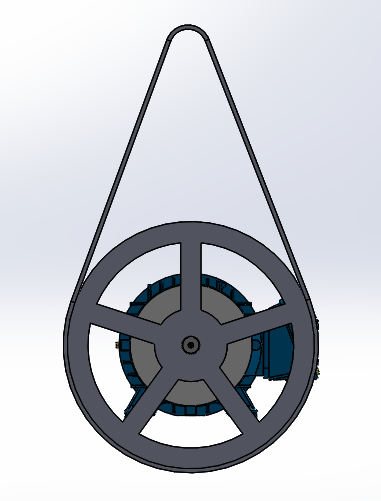
\includegraphics[scale=0.6]{figuras/config_polia.png}
\caption{Configuração do acoplamento polia, motor e correia. Fonte: Autores}
\label{fig:config_polia}
\end{figure}

\subsubsubsection*{\textbf{Mancal e eixo}}

    Fora escolhido como mecanismo de transmissão de movimento deste projeto, mancal e eixo centralizado. Mancal é um componente de uma máquina que possui a função de permitir com que o eixo flutue em uma posição determinada, ou seja, funciona como um suporte ou guia a fim de que o eixo possa ser utilizado sem perdas de desempenho devido ao contato com peças externas.

    A escolha do mancal deve-se ao fato de suas diversas vantagens que se enquadram nos pré-requisitos do projeto tais como: amortecem as vibrações, choques e ruídos, construção simples e custos menores nos projetos dependendo da utilização e finalidade. Os mancais podem ser separados em dois grupos: os de rolamento e os de deslizamento. O que fora escolhido no projeto foi o mancal de deslizamento devido ao fato dele adaptarem-se facilmente as circunstâncias, simples de montar e desmontar e de já o possuirmos.

    Ao se escolher os mancais de deslizamento houve a preocupação de tomar alguns cuidados em relação a sua manutenção, esses são sujeitos as forças de atrito estas por sua vez surgem devido a rotação do eixo que exercerá carga nos apoios, ou seja, deve-se haver um sistema de lubrificação com o intuito de minimizar as perdas pelo atrito

    Os mancais de deslizamentos são constituídos de bucha (corpo cilíndrico oco que envolve o eixo) fixada num suporte, estes mancais são utilizados em máquinas pesadas ou em equipamentos com pouca rotação, pois devido ao atrito os componentes aquecem. Ao se utilizar a bucha e lubrificantes reduzimos o atrito e melhoramos a rotação e consequentemente melhoramos o desempenho da rotação.

    O objetivo em se utilizar este sistema é colocar uma massa desbalanceada com o intuito de que gere na mesa as vibrações desejadas, para que isso ocorre tem que levar em consideração tais observações: Massa desbalanceadora, que se trata de um peso com uma distribuição não uniforme por meio deste podemos obter amplitudes de vibração ou seja quanto maior for a massa desbalanceada maior será a amplitude de vibração; Raio da ação da massa desbalanceadora, pois quanto maior for o raio desta massa maior será a amplitude para a mesma massa desbalanceada; Rotação da polia, em relação a esta podemos analisar que ao se aumentar a rotação aumenta-se a amplitude de vibração de acordo com o desbalanceamento. A Figura\ref{fig:mancal} ilustra melhor o mancal e seu respectivo eixo a ser utilizado no projeto.

\begin{figure}[H]
\centering
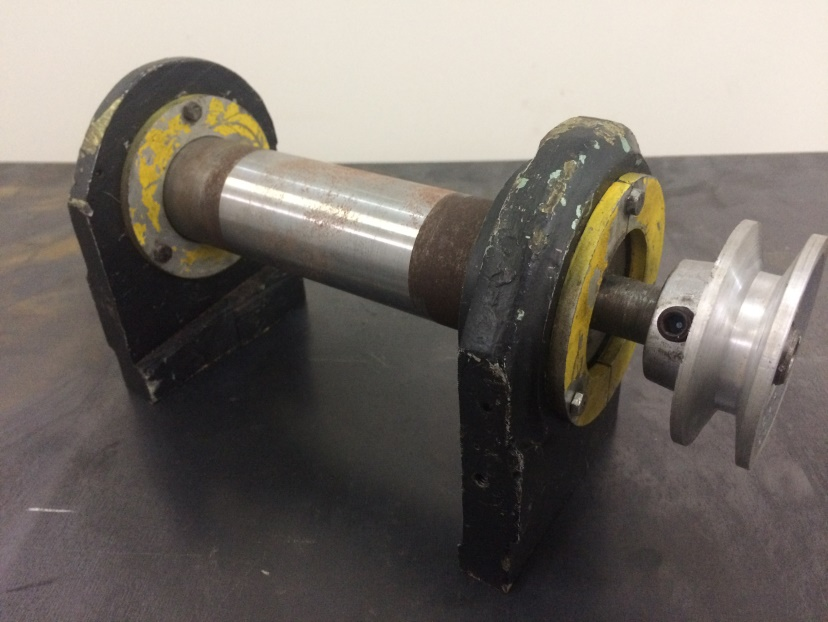
\includegraphics[scale=0.9]{figuras/mancal.jpg}
\caption{Mancal a ser utilizado com seu respectivo eixo e polia acoplados. Fonte: Autores}
\label{fig:mancal}
\end{figure}

\subsubsubsection*{\textbf{Relação polia/eixo}}

    Tendo em vista que a rotação máxima do motor é de 1720 rotações por minuto e que esta rotação equivale apenas a 28,67Hz. Como uma das primícias do projeto visa chegar à vibrações de até 100Hz é necessário aumentar a rotação do motor. Para tal utilizamos uma relação entre polias para que seja possível chegar uma rotação de no mínimo 6000 rotações por minuto o que equivale a uma relação de 3,5. Tendo em vista a polia maior com diâmetro de 250mm é necessário que a polia menor seja de diâmetro máximo de 71,42mm. Entre as polias comerciais a menor mais próxima do valor citado anteriormente equivale a um diâmetro de 60mm atendendo assim as especificações do projeto, podendo assim o eixo fixado na mesa chegar até 7166 rotações por minuto.
